\documentclass{article}
\usepackage{graphicx}
\usepackage[utf8]{inputenc}
\usepackage{subcaption}
\usepackage{amsmath}
\usepackage{tabularx}
\usepackage{mathtools}
\DeclarePairedDelimiter\ceil{\lceil}{\rceil}

\begin{document}

    \section*{Task 1}

    Derive dynamic model for your robot model using the Euler-Lagrange approach

    For this assignment I used the following link model:

    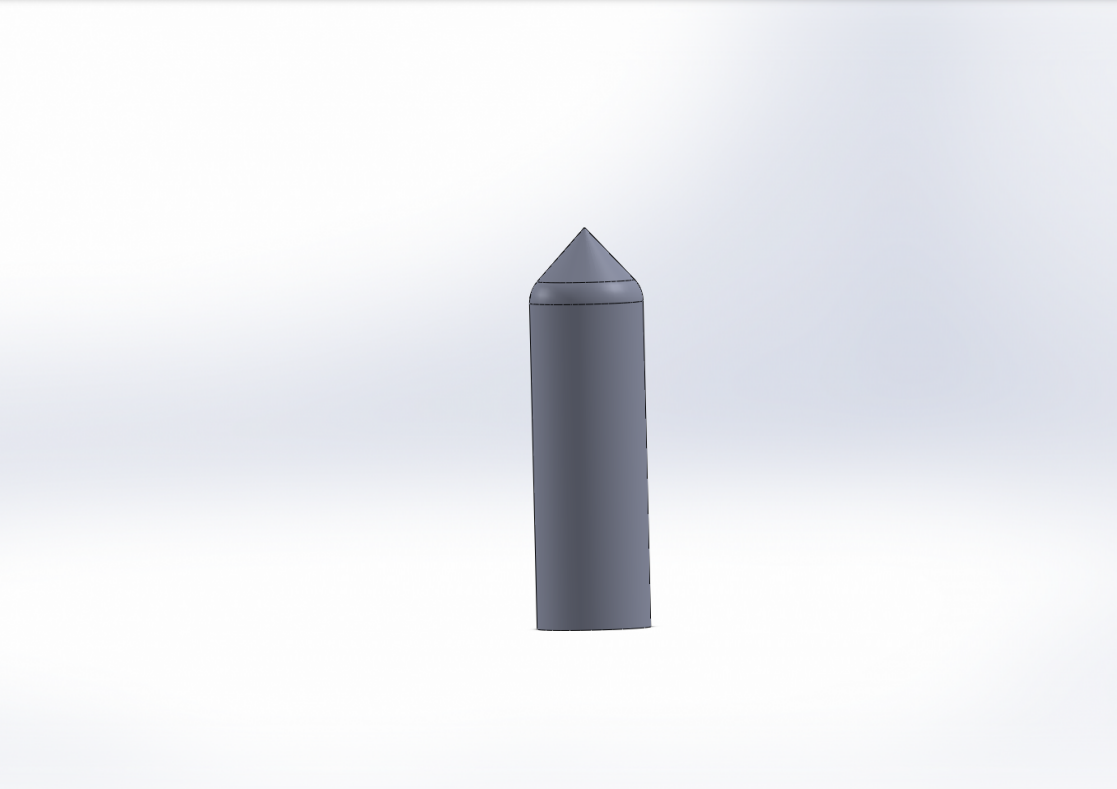
\includegraphics[width=\linewidth]{part_image.png}

    It has mass equal to $111.83\ g$ and inertia tensor $\begin{pmatrix}
        127315.49 & 0 & 0 \\
        0 & 17300.01 & 0 \\
        0 & 0 & 127315.49
    \end{pmatrix}$ given in $\frac{g}{m^2}$

    I took one third of the length of this link as a center of mass. 

    \begin{enumerate}
        \item I found inertial matrix using the formula

            $$M(q) = \sum_{i=1}^{n} m_i J_{v_i}^{T} J_{v_i} + J_{\omega_i}^{T} R_i I R_{i}^{T} J_{\omega_i}$$

        \item Then coriolis matrix:
        
            $$C(q, \dot q) = \sum_{k=1}^{n} c_{ijk} \dot q_k$$
            where $c_{ijk} = \frac{1}{2} (\frac{\partial m_{ij}}{\partial q_k} + \frac{\partial m_{ik}}{\partial q_j} - \frac{\partial m_{jk}}{\partial q_i})$, where $m_{ij}$ are elements of matrix $M$

        \item Gravity vector:
        
            $$g(q) = \sum_{k=1}^{n} (J_{v_i}^k)^T m_k g_0$$
    \end{enumerate}
    
    Using matrices from above, I got dynamic model for the robot:

    $$M(q) \ddot q + C(q, \dot q) \dot q + g(q) = \tau$$

    \section*{Task 2}

    Drive the robot joints between $[0, \pi]$

    With zero velocity and acceleration: 

    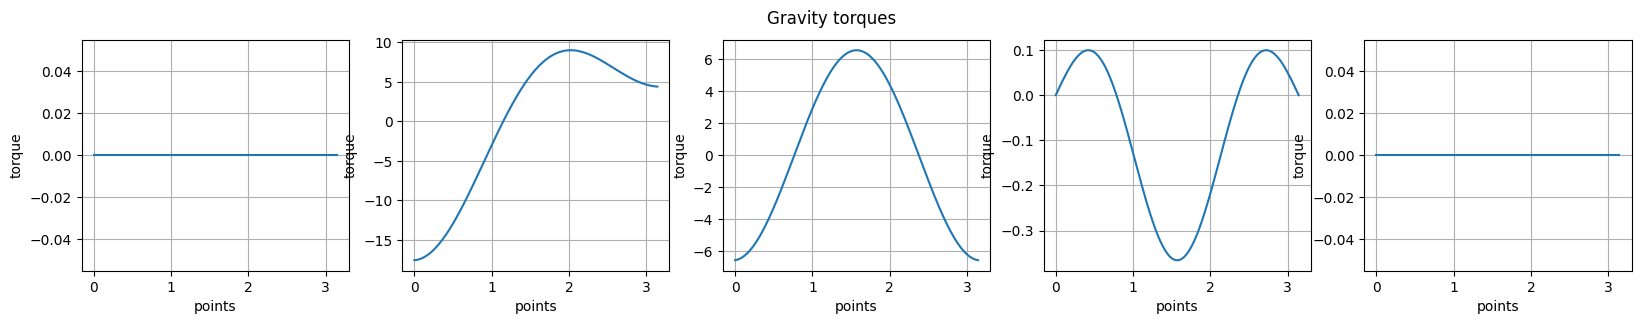
\includegraphics[width=\linewidth]{gravity_torques.png}

    With trapezoidal profile: 

    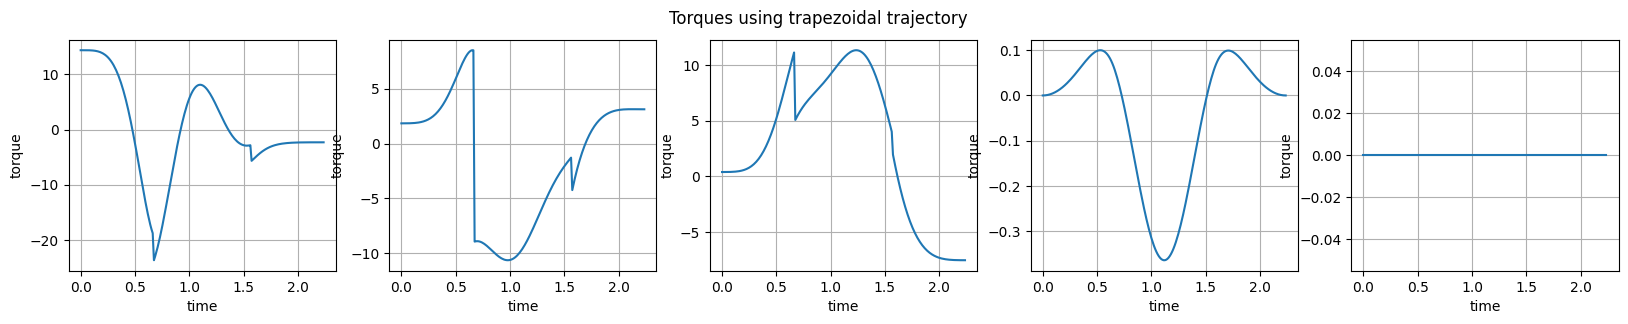
\includegraphics[width=\linewidth]{trapezoidal_torques.png}

    With polynomial profile: 

    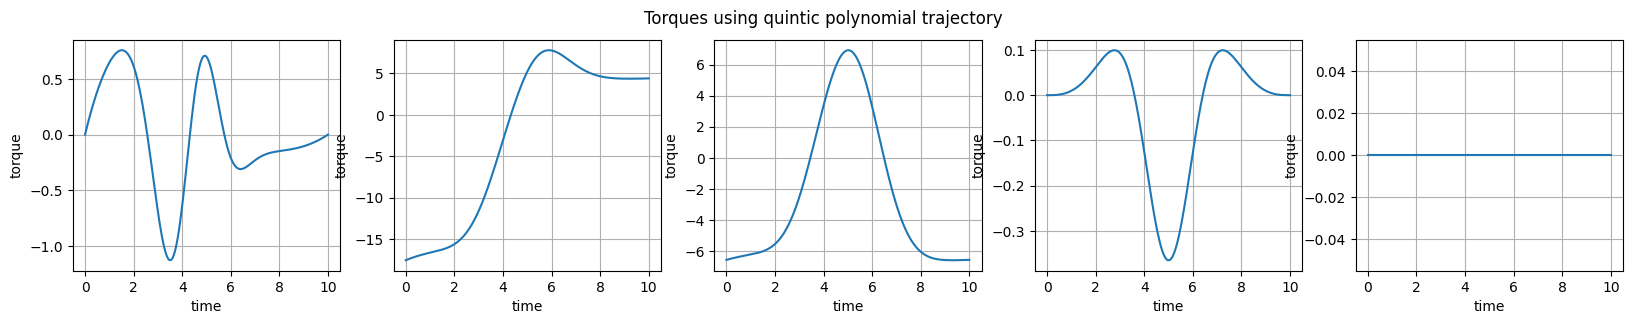
\includegraphics[width=\linewidth]{polynomial_torques.png}

\end{document}